\section{Simulation}
The problem was solved with the provided SEPRAN package. Using the symmetries of the original problem, the domain $\Omega$ as depicted in Figure~\ref{fig:domain_new}, is simulated. First a the mesh was defined, see Figure \ref{fig:empty_mesh}. The mesh is then uniformly filled with triangular elements as seen Figure \ref{fig:filled_mesh}. The commented source code for this mesh is shown in appendix \ref{ap:mesh}.
\begin{Figure}
 \centerfloat
 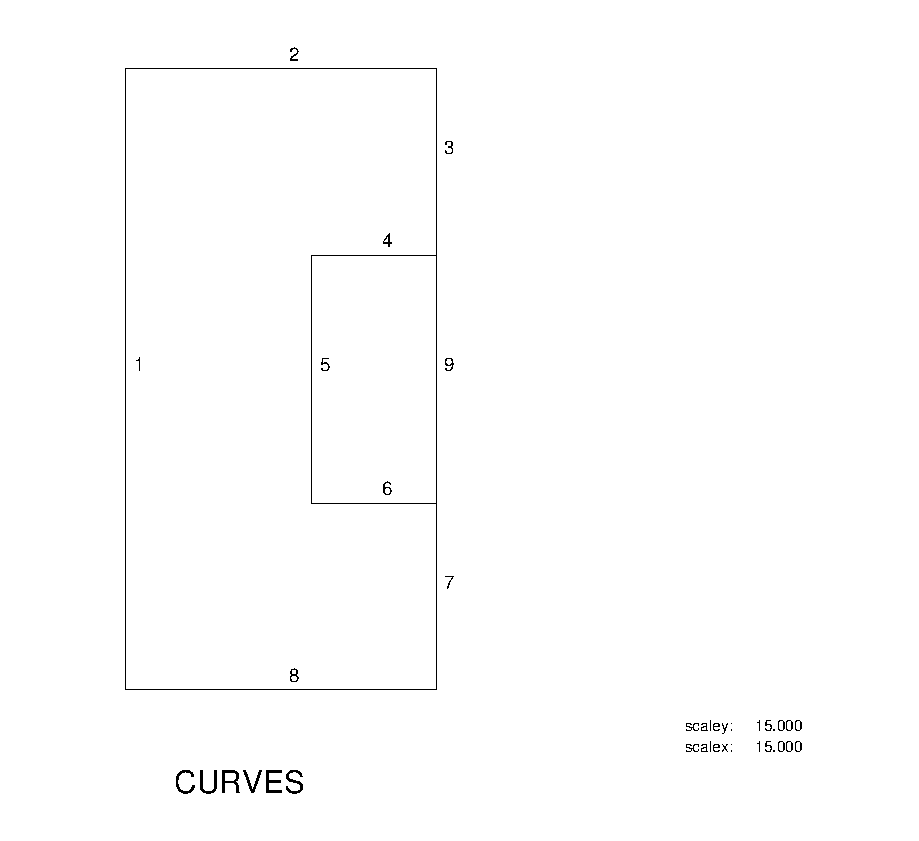
\includegraphics[width=0.4\linewidth, trim=1cm 2cm 7cm 0.5cm, clip]{empty_mesh.eps}
 \captionof{figure}{Mesh boundaries.}\label{fig:empty_mesh}
\end{Figure}~
\begin{Figure}
 \centerfloat
 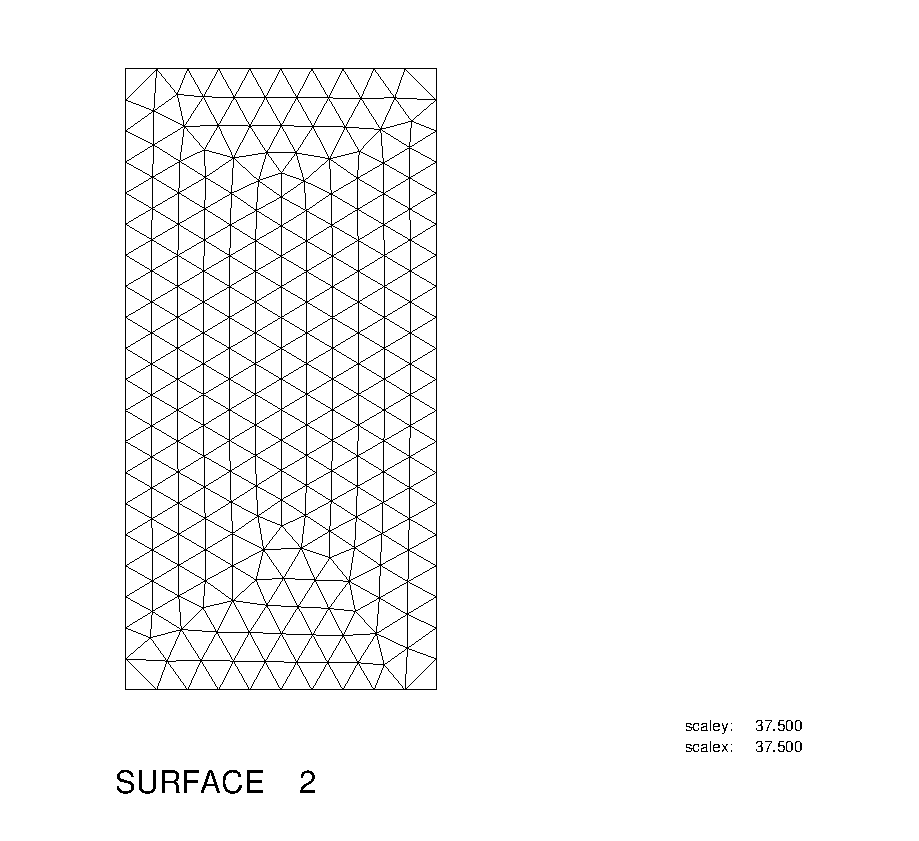
\includegraphics[width=0.6\linewidth, trim=1.5cm 2cm 7.5cm 0.5cm, clip]{filled_mesh.eps}
 \captionof{figure}{Mesh filled with triangular elements.}\label{fig:filled_mesh}
\end{Figure}
A subroutine for the elements was then written. The element matrices and vector for the internal and boundary elements from section \ref{sec:elem} are defined here. The internal elements only have an element matrix, the element vector is set to zero. Generally the boundary elements have an element matrix as well as an element vector. In this simulation however $T_{\infty}=0$, so the boundary element vector is effectively also zero. In the subroutine there is a distinction made between $\Omega_A$ (\texttt{itype==1},~\texttt{itype=3}) and $\Omega_B$ (\texttt{itype==1},~\texttt{itype=3}) for the different heat conductivities $k_A$ and $k_B$. The factors $\beta$, $\gamma$ and $\Delta$ are determined as described in \cite{kan}. The full source code is shown in appendix \ref{ap:elem}.

In a seperate file,  the \texttt{itype} numbers are assigned to the element groups. for the boundary conditions are 

\begin{Figure}
 \centerfloat
 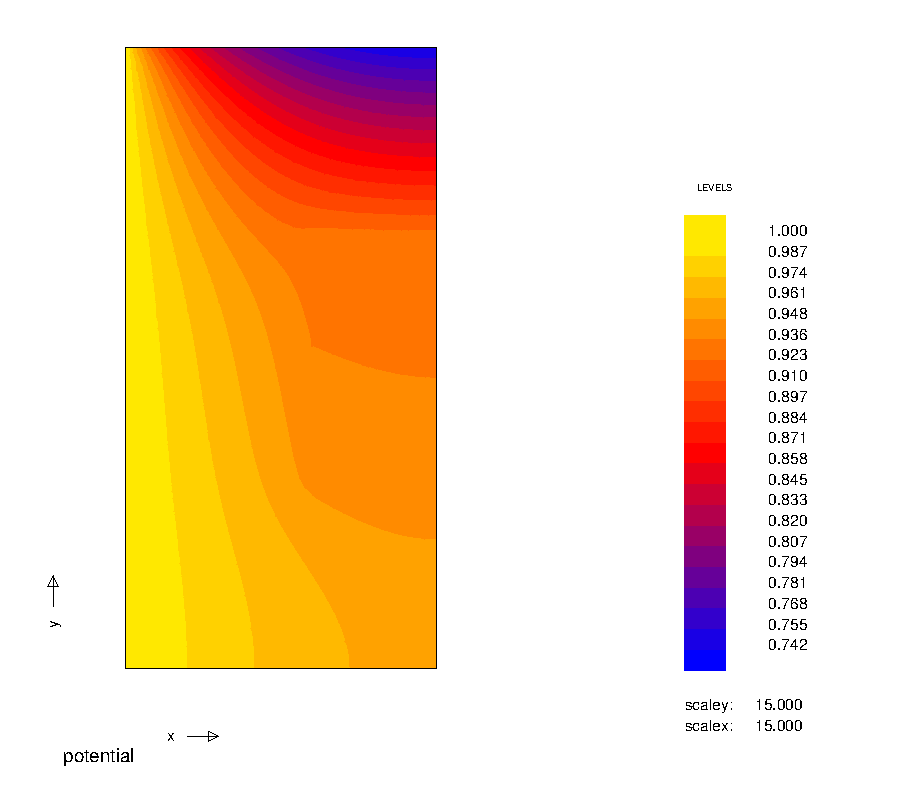
\includegraphics[width=0.8\linewidth]{coef_001.eps}
 \captionof{figure}{Heat distribution for $\alpha = 0.01$.}\label{fig:coef_0.01}
\end{Figure}

\begin{Figure}
 \centerfloat
 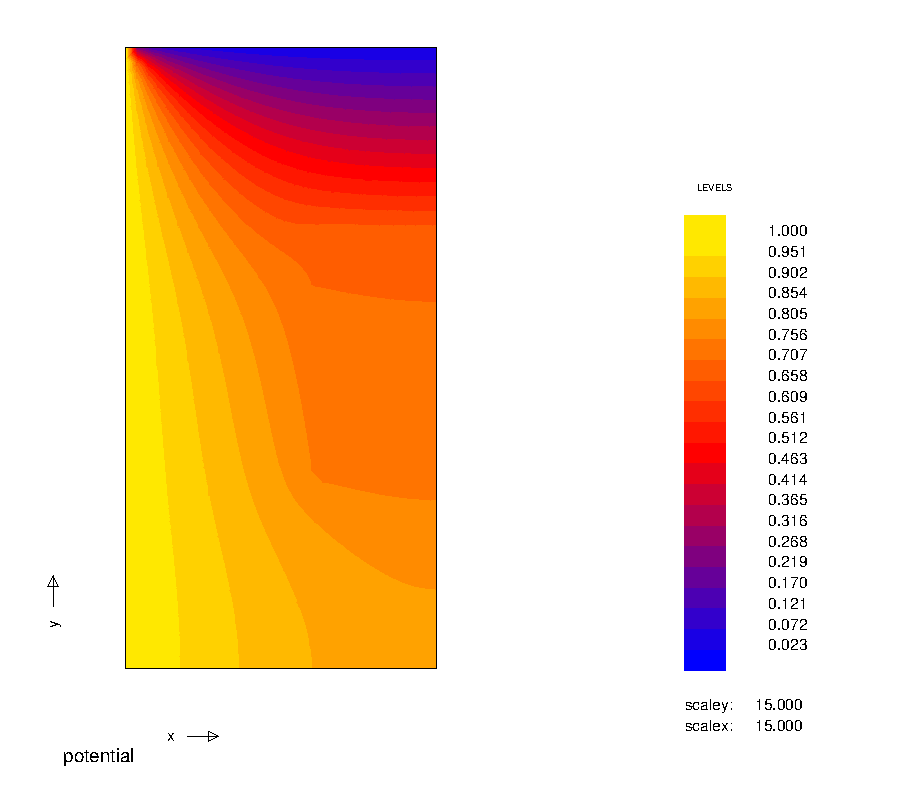
\includegraphics[width=0.8\linewidth]{coef_10.eps}
 \captionof{figure}{Heat distribution for $\alpha = 10$.}\label{fig:coef_10}
\end{Figure}